\chapter{Stand der Technik}
\section{Ultrasound Applikation}
ddas hier ist 

\section{\acs{emi} und mixed-Signal \acs{pcb}}

Die symmetrische Signalübertragung (Störfestigkeit) Seite 140f.
ab 500 \ac{mhz} trägt das filterlayout bei (S190) -> Filterlayout vernachlässigbar
Seite 235 - Kleinrechner boards pi filter..

Gegentakt / Gleichtaktstörungen
Galvanische Kopplung und Gegenmaßnahmen
Kapazitive Kopplung und Gegenmaßnahmen
Induktive Kopplung und Gegenmaßnahmen
Filter
Filterschaltungen (Seite 127f.)
Prinzip, Tiefpass, 
\begin{comment}
\section{Transducer}
Um die elektrische Energie in mechanische Energie und umgekehrt zu wandeln wird ein Transducer benötigt, welches gleichzeitig das Kernstück der Ultraschallsonographie darstellt.\\
Dieser besteht wie in \autoref{Abkuerzungen} gezeigt aus einen oder mehreren Piezoelementen mit der dazugehörigen matching-Schicht für die verbesserte Fokussierung. Da die longitudinal Wellen auf beiden Seiten eines Piezoelementes entstehen, müssen die Wellen auf der Rückseite der Sonde absorbiert werden um Reflektionen zu vermeiden. Dies geschieht durch einen einen akustischen Absorber und einen \textbf{backing block}. Zudem muss die Sonde vor \ac{emi} Störungen geschützt werden, da das Piezoelement auf einstrahlende Frequenzen reagieren kann. Dies geschieht durch ein geschirmtes Metallgehäuse welches an der Messstation geerdet ist und somit die Störungen ableiten kann.\\
Für die Bestimmung der Arbeitsfrequenz $f_0$ kann grundlegend gesagt werden, dass die genierten Frequenzen umgekehrt proportional zur Dicke des Piezoelementes $l_{piezo}$ ist. Um möglichst viel Energie effektiv umwandeln zu können, wird das Piezoelement bei möglichst geringer Impedanz betrieben wobei die Phasenverschiebung 0$^\circ$ beträgt und somit eine reine reelle Last getrieben wird. Dabei ist zu beachten, dass das Element schnellstmöglich ein- und ausschwingen soll, wodurch es am besten in Resonanz betrieben wird. Laut \ref{Abkuerzungen} vibriert ein Piezoelement in Resonanz, wenn die Dicke $l_{piezo}$ gleich $1/2\lambda$ ist, wodurch sich folgende Formel für die Bestimmung der Arbeitsfrequenz $f_0$ eines Piezoelementes aufstellen lässt.
\begin{align}
l_{piezo}&=\frac{1}{2}\lambda =\frac{1}{2} \frac{c}{f_0}\\
f_0&=\frac{c}{2\cdot l_{piezo}}
\end{align}
\subsection*{Kristall-Impedanz-Matching}
Nachdem die zu emittierende Frequenz und somit die Kristalldicke definiert wurde, muss anhand des Impedanz-Frequenz-Diagrammes des ausgewählten Kristalls eine Impedanzanpassung durchgeführt werden. Dieser Schritt ist nötig, da das Schleifen der Kristalle Fertigungstoleranzen unterliegt, und somit nicht genau auf die zu emittierende Frequenz geschliffen werden können. Nachfolgende Gleichung  wird für die Parallelabstimmung genutzt und mit dieser die parallele Induktivität $L_{par}$ bestimmt, wodurch die Breitbandigkeit des Kristalls erhöht wird.
\[L_{par}=\dfrac{1}{\omega_s^2\cdot C_0}\ mit\ \omega_s=2\pi f_s \]
Bild-Ersatzschaltbild RCL || $C_0$ + Bild-Impedanzkurve

\newpage
\section{Auswertung der Ultraschallmessung und Bildentstehung}
\begin{description}\itemsep0pt
\item[A-Mode]\label{a-mode} auch "'Amplitudenmodus" genannt, ist die erste Darstellungsform in der Sonographie und die einfachste Umsetzung des Impuls-Echo-Prinzips. Es ist eine eindimensionale Abbildung der reflektierten Schallwellen in einem Diagramm und stellt die empfangen Echos in Abhängigkeit von der Tiefe dar, wie in Abb. \ref{fig:a_mode} zu sehen ist.
\item[B-Mode]\label{b-mode} auch "Brightness-Mode" genannt, stellt die Echos nicht als Ausschläge, sondern als Bildpunkte mit unterschiedlicher Helligkeit auf dem Bildschirm dar. Dabei entspricht jede Amplitude einem Helligkeits- \ac{bzw} Grauwertbild und ist abhängig von der Intensität der elektrischen Signale\footnote{je stärker das Echo, desto heller der Bildpunkt}. Bei modernen Ultraschallgeräten sind 256 Grauwerte zwischen schwarz und weiß möglich. Ein schwarzes Bild wird dabei durch zu geringe Schallintensität erzeugt, welches die Folge von Totalreflexion oder fehlenden Impedanzunterschied\footnote{keine Reflexion möglich} ist.
\item[M-Mode]\label{m-mode} auch "Motion-Mode" genannt, stellt Gewebestrukturen an einem bestimmten Ort als Funktion der Zeit dar. Dabei werden die Amplituden der Ultraschallechos wie im B-Mode [\ref{b-mode}] aber zu einem bestimmten Zeitpunkt dargestellt. Über ein Ort-Zeit-Diagramm werden örtliche Veränderungen echogener Strukturen über die Zeit dargestellt\footnote{Time-Motion Verfahren}, wie in Abb. \ref{fig:m_mode} zu sehen ist. Dabei wird die Amplitude auf der vertikalen Achse und die von den wiederholten Impulsen erzeugten Echos auf der horizontalen Achse (Zeitachse) abgetragen.
\item[Doppler Spektrogramm]\label{spektrogramm} ist eine Darstellung, wobei auf der X-Achse die Zeit und auf der Y-Achse die Frequenzverteilung dargestellt sind. Da die dargestellten Frequenzen abhängig der Fließgeschwindigkeit der Blutteilchen sind, können Aussagen über die Durchschnittsgeschwindigkeit des Blutes, sowie über Schlagvolumen und Herzfrequenz gemacht werden (visualisiert in Abb. \ref{fig:m_mode}). Dies ist mithilfe der Kurzzeit-Fourier-Transformation (eng: short-time Fourier transform, STFT) realisierbar, in der kurze Zeitabschnitte in den Spektralbereich überführt werden.
\end{description}
\begin{figure}[ht]
  \centering
  \begin{subfigure}[b]{0.48\textwidth}
	\centering
  	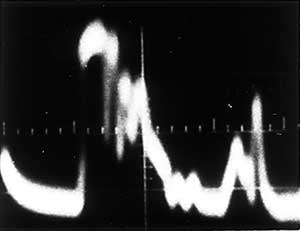
\includegraphics[height=4cm, width=\textwidth]{A-Mode}  
  	\caption{A-Mode}
  	\label{fig:a_mode}
  \end{subfigure}
  \hfill
  \begin{subfigure}[b]{0.48\textwidth}
	\centering
  	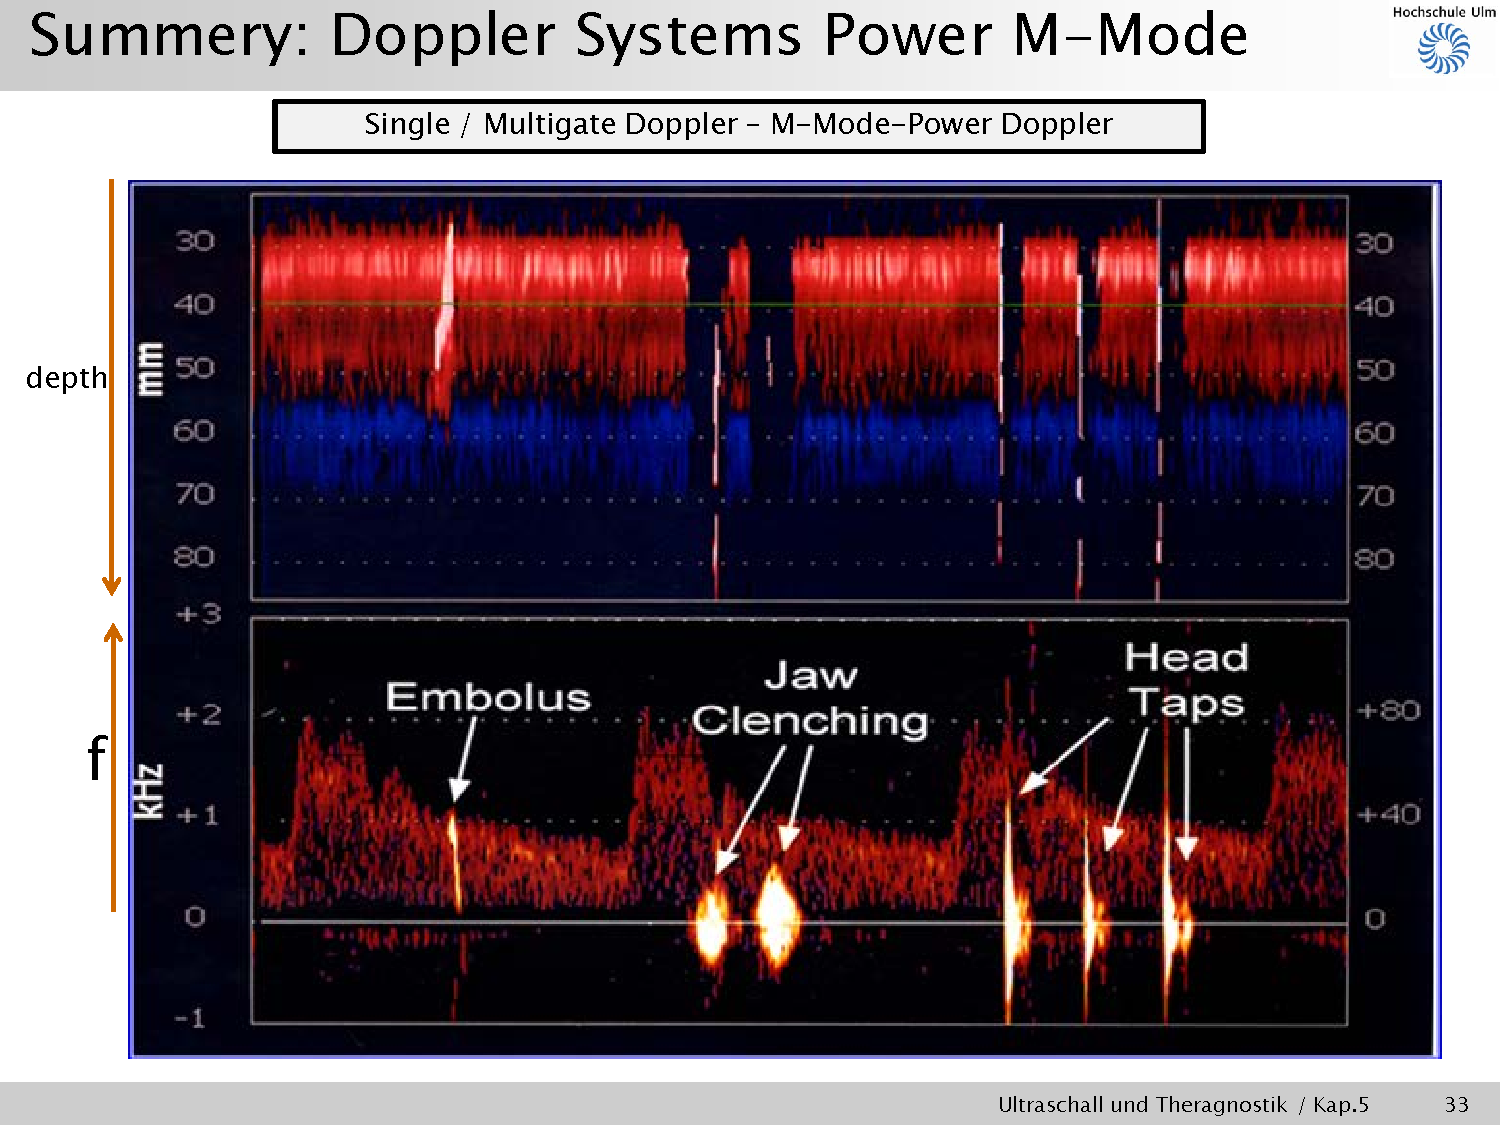
\includegraphics[trim = 2.2cm 1cm 1.3cm 3.5cm, clip=true,height=4cm, width=\textwidth]{M-Mode}  
  	\caption{M-Mode mit Doppler Spektrogram}
  	\label{fig:m_mode}
  \end{subfigure}
  \caption{Modes der Bildentstehung}
  \label{fig:modes}
\end{figure}
\newpage
\section{Methoden der Emboliedetektion}
blablabla
\end{comment}
